\documentclass[11pt]{article}
\usepackage[a4paper,margin=25mm,top=22mm,bottom=22mm]{geometry}
\usepackage{amsmath,amssymb,amsthm,mathtools,booktabs,array,graphicx,xcolor,hyperref,microtype,fancyhdr}
\definecolor{ink}{HTML}{183448}\hypersetup{colorlinks=true,linkcolor=ink,citecolor=ink,urlcolor=ink,pdfauthor={},pdftitle={Uniform average mixing on paths}}
\newtheorem{theorem}{Theorem}\newtheorem{lemma}[theorem]{Lemma}\newtheorem{corollary}[theorem]{Corollary}
\theoremstyle{remark}\newtheorem*{remark}{Remark}
\newcommand{\E}{\mathbb E}\newcommand{\R}{\mathbb R}\newcommand{\Z}{\mathbb Z}\newcommand{\Q}{\mathbb Q}\newcommand{\T}{\mathbb T}\newcommand{\abs}[1]{\left|#1\right|}\newcommand{\norm}[1]{\left\|#1\right\|_1}
\DeclareMathOperator{\conv}{conv}\DeclareMathOperator{\ri}{ri}\DeclareMathOperator{\diag}{diag}\DeclareMathOperator{\Rea}{Re}
\pagestyle{fancy}\fancyhf{}\fancyhead[L]{\small Uniform average mixing on paths}\fancyhead[R]{\small Research preprint v0.1.0}\fancyfoot[C]{\thepage}\setlength{\headheight}{15pt}\setlength{\parindent}{1.2em}\setlength{\parskip}{1.5pt}\allowdisplaybreaks

\title{\vspace{-1.2em}\bfseries Uniform Average Mixing on Path Graphs:\\ An Arithmetic Classification via Positive Fourier Densities}
\author{}\date{27 November 2026 \quad $\cdot$ \quad Research preprint v0.1.0}
\begin{document}\maketitle
\begin{center}\small AI-assisted research manuscript; candidate proof, not peer reviewed.\end{center}
\begin{abstract}
For the continuous-time adjacency quantum walk on the path $P_N$, uniform average mixing asks whether a single probability law for the readout time produces the matrix $J_N/N$. Writing $q=N+1$, Kang established the obstruction when $15\mid q$, $21\mid q$, or $6\mid q$ with $q\ge12$, and proved existence for prime, twice-prime and power-of-two moduli. We present a candidate proof that these obstructions are exhaustive. The proposed positive direction constructs positive Fourier densities on the compact cyclotomic phase group. Low-degree moment identities and a classification of short signed root-of-unity relations bound the corrections to the independent-circle or three-coordinate-block model. The thirteen finite even cases and the formerly LP-dependent case $q=33$ are handled by exact rational Fourier computations; the other small odd cases are treated separately. The construction also yields finite readout laws on arbitrary algebraic-step time grids, a uniform Haar component of size $1/100$, and a conditional timing-noise compensation bound. Detailed arithmetic inventories, executable verification scripts, and audit records accompany the manuscript. The full proof has not undergone independent peer review or Lean formalization.
\end{abstract}
\noindent\textbf{Keywords:} continuous-time quantum walk; uniform average mixing; cyclotomic fields; Fourier moments; convex geometry.\par
\section{Introduction and statement of results}
Let $A$ be the adjacency matrix of the path on $N\ge2$ vertices. Its transition-probability matrix is $M(t)=|e^{itA}|^{\circ 2}$, where $\circ$ denotes entrywise operations. For a Borel probability measure $\mu$ on $\R$, define
\begin{equation}\label{eq:mix} \widehat M[\mu]=\int M(t)\,d\mu(t).\end{equation}
Uniform average mixing (UAM) means $\widehat M[\mu]=J_N/N$ for every initial site simultaneously. This differs from instantaneous mixing and the Ces\`aro limit \cite{godsil}. Baptista, Coutinho and Marques introduced random-time averaging and supplied small path examples \cite{baptista}. Kang subsequently characterized the forced cosine coherences and classified parity collisions \cite{kang}. The absence of a collision is a necessary consistency condition; it is not by itself a probability-law construction.

\begin{theorem}[Candidate arithmetic classification]\label{thm:main}
For $q=N+1\ge3$, $P_{q-1}$ admits UAM if and only if
\begin{equation}\label{eq:arithmetic}15\nmid q,\qquad21\nmid q,\qquad (6\nmid q\ \text{or}\ q=6).\end{equation}
For each admitted $q$, any algebraic $\delta>0$ and any $t_0\ge0$, a realizing law can be chosen on a finite subset of $t_0+\delta\Z_{\ge0}$. With $m=\lfloor(q-1)/2\rfloor$, the support size is at most $m^2+1$ for odd $q$, and $m(m+1)+1$ for even $q$.
\end{theorem}
The necessity in Theorem~\ref{thm:main} is due to Kang (Theorem S18 of \cite{kang}); the proposed contribution is the remaining sufficiency. The constructive cases are partitioned into (I) odd $q$ coprime to $3$, (II) odd $q$ divisible by $3$ but coprime to $35$, and (III) even $q$ coprime to $3$. The small case $q=6$ is already known. Figure~\ref{fig:class} illustrates the classification. The detailed proof and all arithmetic tables are in the companion file \texttt{detailed-proof.md}, denoted DP below; it is part of the proof, not optional evidence. The proofs of the local relation inventories in DP are essential to the general theorem.
\begin{figure}[ht]\centering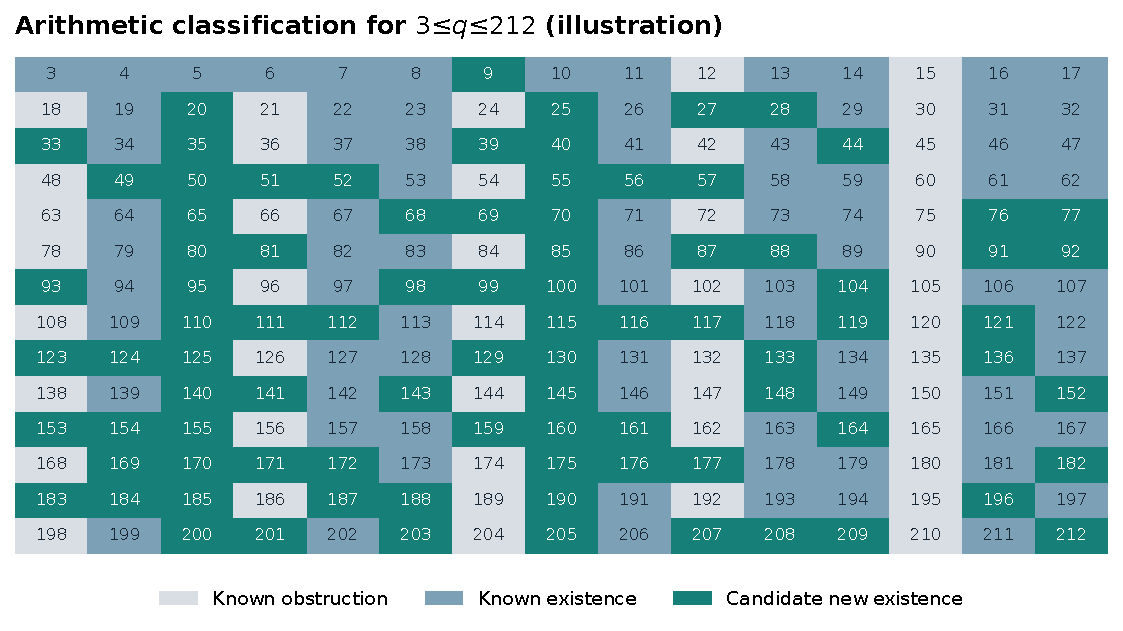
\includegraphics[width=.98\linewidth]{../figures/classification.pdf}\caption{Arithmetic status of the first 210 moduli starting at $q=3$. Prior existence and obstruction classes follow \cite{kang}; the dark class is the proposed extension. This illustration is not an exhaustive proof.}\label{fig:class}\end{figure}
\section{Spectral reduction and the phase moment problem}
The eigenvalues and real unit eigenvectors are
\begin{equation}\theta_r=2\cos(r\pi/q),\quad v_r(k)=\sqrt{2/q}\sin(rk\pi/q),\quad E_r=v_rv_r^{\mathsf T},\quad 1\le r,k\le q-1.\end{equation}
Let $S$ denote the reversal matrix, $I$ the identity and $J=J_N$. Since $A$ is real symmetric,
\begin{align}M(t)&=D_0+2\sum_{r<s}\cos[(\theta_r-\theta_s)t]E_r\circ E_s,\\D_0&=\sum_r E_r\circ E_r=\frac{2J+I+S}{2q}.\end{align}
The two reflection parity projectors are $(I\pm S)/2$. The sum of their entrywise squares is $(I+S)/2$. Consequently the target
\begin{equation}\label{eq:target}y_{rs}=\begin{cases}-1/N,&r\ne s,\ r\equiv s\pmod2,\\0,&r\not\equiv s\pmod2\end{cases}\end{equation}
gives $D_0-N^{-1}[(I+S)/2-D_0]=J/N$. Kang proves that these coherences are forced, and that collisions between opposite target classes occur precisely at the forbidden moduli \cite[Sections S2--S3]{kang}.

Let $\alpha\in\R^m$ be the chosen nonzero representative energies, one per pair $\theta,-\theta$. For odd $q$, use $\alpha_j=2\cos(2\pi j/q)$, $j=1,\dots,m$ (these need not be positive); for even $q$, use $\alpha_j=\theta_j$, $1\le j<q/2$. Write $z_j=e^{i\phi_j}$ and
\begin{equation}H=\overline{\{t\alpha\bmod2\pi:t\in\R\}}\subseteq\T^m,\qquad \Lambda=\{c\in\Z^m:c\cdot\alpha=0\}.\end{equation}
With $h$ normalized Haar measure, $\int_H z^c\,dh=\mathbf1_{c\in\Lambda}$. The problem is to find a positive phase law with prescribed real character moments, then pass to actual times.
\begin{lemma}[Fourier correction]\label{lem:correction}
Let $V$ contain nontrivial characters, pairwise distinct up to inversion on $H$. For a real nonnegative Fourier polynomial $F$, let $Z_H=\E_hF$ and $M_v=\E_h(F\Rea z^v)$. Given real targets $y_v$ and $T>0$, the function
\begin{equation}\label{eq:correction}f=\frac{F+T-Z_H+2\sum_{v\in V}(Ty_v-M_v)\Rea z^v}{T}\end{equation}
has mass one and target moments. It is strictly positive if $T-Z_H>2\sum_v|Ty_v-M_v|$.
\end{lemma}
\begin{proof}Distinct real character cosines have Haar mean zero and mutual inner products $\delta_{uv}/2$. Integrate (\ref{eq:correction}) and its products with each target cosine; the lower bound follows from $F\ge0$ and $|\Rea z^v|\le1$.\end{proof}
\section{Short cyclotomic relations}\label{sec:relations}
Only Fourier monomials of length $\norm c\le10$ occur in the moments below. The corresponding signed root array has total absolute weight at most 20 and no coefficient at the excluded fixed points. Its support is at most its absolute weight. Partition the support into inclusion-minimal vanishing subsets, retaining the original coefficients, without requiring the partition to respect inversion. By the signed rational Conway--Jones theorem \cite[Theorem 5]{cj} (see also \cite[Theorem 2.6]{lenstra}), each subset lies in a coset of a subgroup of squarefree reduced order $d$ and has at least
\begin{equation}\label{eq:cj}2+\sum_{p\mid d}(p-2)\end{equation}
nonzero terms. A prime-order subset is a complete prime cycle with constant coefficient by irreducibility. In the even case fold exponents modulo $q$ with $\zeta^{j+q}=-\zeta^j$, $\zeta=e^{i\pi/q}$. The chosen exponents $\pm r$, $0<r<q/2$, are distinct modulo $q$; folding preserves support. The projected squarefree order is odd, and the factor 2 in (\ref{eq:cj}) contributes zero.

A stable odd-order coset under inversion has exactly one fixed point, $0$ for odd $q$, and $0$ or $q/2$ for even $q$. Both are excluded in the root array. The even central lifts have factors $1$ and $i$, producing symmetric and antisymmetric coefficients respectively. A subset with support $>10$ must be central since its inverse coset would otherwise require another $>10$ entries. This reasoning concerns the whole array, not a symmetric minimal partition.

There is an independent algebraic localization. Let $d$ be the odd radical of $q$ and $a=q/d$. Then $\Phi_q(x)=\Phi_d(x^a)$ for odd $q$ and $\Phi_{2q}(x)=\Phi_{2d}(x^a)$ for even $q$. Decompose a folded root array $A(x)=\sum_{j=0}^{a-1}x^j A_j(x^a)$. Divisibility holds exactly when each $A_j$ is divisible by the corresponding radical polynomial. In squarefree order $d=pr$, evaluate each $p$-row at a primitive $r$th root. Irreducibility of $\Phi_p$ over $\Q(\zeta_r)$ makes the row evaluations equal. If $p>20$, some row is empty, so all vanish. Iteration removes such primes. These classical reductions do not alone establish the required inventories; the minimal-support bound and the case analysis below supply the remaining restrictions.

\begin{lemma}[Short relation inventories]\label{lem:inventory}
For odd $q$ with $3\nmid q$, all nonzero relations relevant to charge-zero polynomials of degree eight have even length at most 10 and charge $Q(c)=\sum_i c_i\in\{0,\pm2\}$. Their six types are given in Table~\ref{tab:odd}. For odd $q$ divisible by 3 but coprime to 35, the baseline lattice consists of vectors constant on each triple and zero on a singleton; additional relevant relations have charge $\pm2$ and occur only at reduced orders 33 and 39. For even $q$ coprime to 3, each parity group has the absolute-pattern bounds in Table~\ref{tab:even}. In these three settings the target cosines are nontrivial and mutually orthogonal.
\end{lemma}
\begin{proof}[Proof outline with exact inventories]
The full enumeration-free local arguments and tables are in DP, Part I, Section 3; Part II, Section 4; and Part III, Section 4. We summarize their reduction and the most restrictive cases. With primes at least 5, (\ref{eq:cj}) permits mixed orders only $35,55,65,77,85,91,385$. With primes 3 or at least 11 it permits $33,39,51,57$. Pure prime cycles pair under inversion: if the inverse of a cycle of length $p\ge5$ were not a same-prime block, its intersection with each of at most three remaining distinct-prime cycles would have at most one root, insufficient to cover it. For the three-block model large prime cycles are ruled out by the weight budget.

For $d=pr$, the kernel of evaluation in CRT coordinates is exactly the additive arrays $A_{ij}=a_i+b_j$, since row and column cycles span dimension $p+r-1=pr-\varphi(pr)$. At the center normalize $a_0=b_0=0$. If the nonzero axis supports have sizes $u,v$, the root support is at least $u(r-v)+(p-u)v$. For symmetric arrays $u,v$ are even. For antisymmetric arrays the intersections add at least $uv/2$. For $d\in\{55,65,77,85,91\}$ the latter exceeds 20. In the symmetric case the only possible nonzero-axis patterns are $(4,8),(4,10)$ for $55$, $(4,12)$ for $65$, $(6,10)$ for $77$, $(4,16)$ for $85$, and $(6,12)$ for $91$. There is space for at most one nonzero paired intersection (cost four); the rectangle identity excludes exactly one. Thus all active row values are $A$, all active column values $-A$, with $|A|=1$. This yields the central counts in the tables.

For order 35, the central symmetric length is
\[L=|a_1|+|a_2|+\sum_{j=1}^3(|b_j|+2|a_1+b_j|+2|a_2+b_j|).\]
If $a_1\ne a_2$, $L\le10$ implies (up to sign and permutation) $(a_1,a_2)=(0,1)$, and each $b_j\in\{0,-1\}$. If equal, the common value is $\pm1$ or $\pm2$ (or zero for pure cycles). For common value 1 the baseline $b_j=-1$ may have at most one replacement by 0 or $-2$; for value 2 all are $-2$. For the antisymmetric case the column cost is $|b|+2\max(|a_1|,|b|)+2\max(|a_2|,|b|)$, which forces exactly one unit row and one unit column when both axes are nonzero. This gives 44 symmetric and 24 antisymmetric mixed arrays. A noncentral mixed 35-coset and its inverse consume the full 20-root budget, forcing a single exceptional row and column, with ten unit entries in each. A central mixed component of length five may coexist with one pure inverse pair of 5-cycles; this is included in Table~\ref{tab:even}.

For $385=5\cdot7\cdot11$, (\ref{eq:cj}) requires at least 19 terms, hence exactly 20 unit entries by inversion. All eleven $5\times7$ slices have the same nonzero evaluation; at least two are singletons. In the antisymmetric case the common value would be purely imaginary, impossible for a signed odd-order root. In the symmetric case normalize the common real value to 1. Singleton slices are at the origin. Other slices require at least four entries. The central slice has even support and no origin, so only central length four with an inverse pair of four-entry slices, or central length ten, is possible. The former reduces the order to 55 (each exceptional slice minus the origin is a 5-cycle); the latter has additive axes with $a_i\in\{0,1,2\}$, $b_j\in\{-1,0,1\}$ and would require half-weight five. If an $a_i=2$ the half-weight is at least ten; otherwise it is $2+5k$, at least seven, or $3+3k$ according to the two row values, never five. This excludes 385. DP gives the charge filter and the full count for each model. No nonzero relevant relation of length at most four can occur; in the triple model the only short relations have length three and cannot identify two length-two target characters (their difference has even length). This proves the claimed orthogonality.
\end{proof}
\begin{table}[ht]\centering\small\caption{Odd $q$, $3\nmid q$: relevant relation types (DP Part I). Counts in the charge $+2$ orientation unless indicated.}\label{tab:odd}\begin{tabular}{llll}\toprule Type & Origin & Length, charge & Count bound\\\midrule I & paired 5-cycles & $10,0$ & $m^2/25$ (both signs)\\II & central 77 & $8,\pm2$ & 1\\III & central 55 & $10,\pm2$ & 5\\IV & noncentral 35 & $10,\pm2$ & $m$\\V & central 35 & $8,\pm2$ & 6\\VI & central 35 (double) & $10,\pm2$ & 1\\\bottomrule\end{tabular}\end{table}
\section{Positive density constructions}\label{sec:density}
\subsection{Odd moduli coprime to 3}
For odd $q$ the target index set $V$ consists of $e_i-e_j$ ($i<j$) and $e_i+e_j$ ($i\le j$). The target is $-1/(2m)$ for the first set and zero for the second. Use
\begin{equation} X=\frac{1}{m}\left|\sum_j z_j\right|^2,\qquad F=(100-60X+7X^2)^2.\end{equation}
On the independent torus, write $Z=\E_*F$, $Y=\E_*XF$. The moments follow from
\[\E_*X^k=\frac{(k!)^2}{m^k}[t^k]\left(\sum_{j=0}^k\frac{t^j}{(j!)^2}\right)^m.\]
Permutation and rotation invariance give conjugate moments $(Y-Z)/(m-1)$ before normalization and zero ordinary moments. Set $T=2m(Z-Y)/(m-1)$. For $m\ge3$,
\begin{align}Z&=4136-968/m+658/m^2-1617/m^3,\\G=T-Z&=\frac{3}{m^3}(232m^3+2568m^2-5782m+15435)\ge696.\end{align}
Here $0<Z<4210$. For charge-zero $u$ of length $2h$, the coefficient of $X^j$ is
\begin{equation}\label{eq:coef}\frac{(j!)^2}{m^j}\sum_{\substack{\ell_i\ge0\\\sum\ell_i=j-h}}\prod_i\frac{1}{(u_i^++\ell_i)!(u_i^-+\ell_i)!}.\end{equation}
It follows that $|\widehat F(u)|\le58464/m^3$ for $h=3$, $28224/m^4$ for $h=4$, and zero for $h>4$. The actual Haar deviations $E_v$ from the independent moments are sums of $\widehat F(c-v)$ over nonzero $c\in\Lambda$. The mass deviation vanishes by the charge-zero length restriction. Counting the permitted cancellations of $v$ in Table~\ref{tab:odd} gives
\begin{equation}E=2\sum_v|E_v|\le\frac{56448}{m^2}+\frac{11007360}{m^3}+\frac{4572288}{m^4}.\end{equation}
Without $35\mid q$ the last two numerators reduce to $1451520,4233600$. For $q\ge55$ not divisible by 35 this is $<160$; for $35\mid q$, $q\ne35$ it is $<25$; for $q<55$, $q\ne35$ only $q=25$ has a pure contribution, bounded by 392. For $q=35$ exact evaluation of (\ref{eq:coef}) gives $E=31239432/83521<375$. Thus $E<G$, and Lemma~\ref{lem:correction} supplies the law. The known small prime cases are covered by \cite{kang}.
\subsection{Odd moduli containing 3 but coprime to 35}
Let $m=3b+1$, $b=(q/3-1)/2$. The inverse pairs of noncentral cosets of the order-3 subgroup give triples with $z_1z_2z_3=1$; the central coset leaves one singleton. Retain every triple constraint in the auxiliary product phase group $H_3$. Use the same $F$ as above. Denote its model mass by $Z$, within-triple, cross-triple and triple-singleton moments by $U,V,W$ respectively. The coefficient extraction in DP Part II, Section 3 gives
\begin{align*}m^4 Z&=335016b^4+414504b^3+122490b^2+126705b+2209,\\m^4 U&=-8(8154b^3+9171b^2+21603b-14243),\\m^4 V&=-24(2718b^3+1857b^2+11035b-21989),\\m^4 W&=-8(8154b^3+9171b^2+21015b-13655).
\end{align*}
The factors of the generating series are sums over multinomial exponents with the difference constant on each triple (zero on the singleton). Put $T=-2mV$, $G=T-Z$. For $b\ge4$, the base correction is $E_b=6b(2V-U-W)$; $V-U,V-W>0$ by their explicit quadratics. At $b=4+x$,
\[m^4(G-E_b)=56376x^4+539784x^3+3753414x^2+10792767x+2172683>0.\]
For the additional relations, a central $3\times r$ array has coordinates $t$ and $(d_j,t+d_j,t+d_j)$, $1\le j\le R=(r-1)/2$. Nontrivial mixed arrays force $t=1$ up to sign, and $d_j\in\{-2,-1,0,1\}$. At most one outside 3-cycle pair is allowed. For $t=1$ write $n_{-2},n_0,n_1$ for counts relative to all $d_j=-1$. Then $L=R+1+3n_{-2}+n_0+4n_1$ and $Q=1-R-3n_{-2}+3n_0+6n_1$. Add length 3 and charge $\pm3$ for an outside pair. Substitution of $R=5,6,8,9$ yields the following table (sign reversed if necessary):
\begin{center}\small\begin{tabular}{llllr}\toprule $r$ & exceptional columns & outside sign & $(L,Q)$ & count\\\midrule 11 & two $0$ & none & $(8,2)$ & 10\\11 & one $1$ & none & $(10,2)$ & 5\\11 & one $0$ & $+1$ & $(10,2)$ & 5 per triple\\13 & one $0$ & none & $(8,-2)$ & 6\\13 & none & $+1$ & $(10,-2)$ & 1 per triple\\17,19 & none admissible & -- & -- & 0\\\bottomrule\end{tabular}\end{center}
Thus no additional charge-zero moments are affected. The extra ordinary-product correction obeys $E_{\rm extra}\le24917760/m^3+2257920/m^4$. When 11 or 13 divides $q>39$, $b\ge16$; at $b=16+x$ the numerator of $G-E_b-E_{\rm extra}$ is bounded below by
\[56376x^4+3245832x^3+71894502x^2+648979023x+1550708831>0.\]
For $q=39$ the exact margin is $9760481/130321$. For $q=33$ complete the square: with triple sum $s_j$, singleton $z_0$, $A_c=V-U=42107/4096$ and $B_c=V-W=40931/4096$,
\[A_c(|s_j|^2-3)+2B_c\Rea(s_j\bar z_0)\ge-3A_c-B_c^2/A_c.\]
The resulting exact margin is $42831862673/172470272>0$. These finite computations use (\ref{eq:coef}) and exact lattice relations, not a numerical LP. The density is (\ref{eq:correction}) with $T=-2mV$. For $q=9$, select an aligned triple of uniform cube roots with probability $5/21$ or a random permutation of the three cube roots otherwise. In the aligned event the singleton is opposite the common root with probability $3/5$, uniform otherwise; in the balanced event it is uniform. All conjugate off-diagonal moments are $-1/7$, ordinary moments vanish by cube rotation, and mixture with Haar of weight $1/8$ yields $-1/8$. The actual phase group equals the triple model by real-field dimension three. The case $q=3$ is known.
\subsection{Even moduli coprime to 3}
For $q=2h$, the automorphism $\zeta\mapsto-\zeta$ sends $\theta_r\mapsto(-1)^r\theta_r$. Thus every rational relation splits into parity parts and $H=H_0\times H_1$. Let $b=1$ for the group of the zero mode, $b=0$ for the other, and $n$ be the group size. Here $N\ge4n-1$ for $b=0$, $N\ge4n+1$ for $b=1$. Required moments are $\E\cos\phi_i=-b/N$ and $\E\cos2\phi_i=\E\cos(\phi_i\pm\phi_j)=-1/N$. Independent conjugation-invariant group laws give cross-parity moments zero. Define
\begin{align}S_0&=\sum_i\cos\phi_i,\quad T_2=\sum_i\cos2\phi_i,\quad X=2(S_0+b/2)^2/n,\\F&=(10000-3707X+254X^2-1336T_2/n)^2.\end{align}
Let $Z,U,D,W$ denote independent-circle mass, distinct cosine-product moment, doubled-angle moment and first moment. They are evaluated symbolically by the marked series
\[B_j(t,u)=\sum_{k\le8,\ell\le2}\frac{t^ku^\ell}{k!\ell!}\E[C^k(2C^2-1)^\ell\cos(j\phi)],\quad C=\cos\phi.\]
Multiply the corresponding products $B_0^n$, $B_0^{n-2}B_1^2$, $B_0^{n-1}B_2$, $B_0^{n-1}B_1$ by $e^{bt/2}$ and extract the coefficients prescribed by $F$. The elementary identity $\E[C^ke^{ij\phi}]=2^{-k}\binom{k}{(k-j)/2}$ (zero for invalid index) gives all coefficients. DP Part III, Section 3 lists the four rational functions for each bias. In particular, with $T=-NU>0$, $G=T-Z$, exact shifted polynomial coefficients establish for all $n\ge2$,
\begin{equation}\label{eq:evenbase}G-2n(|U-D|+|bU-W|)>14500000.\end{equation}
The underlying cosines are $e_i,2e_i,e_i\pm e_j$. A nonzero short relation contributes at most the sum of $|\widehat F(c-v)|$ over all $v$ of length at most two, including zero. Table~\ref{tab:even} records upper bounds; $E_l$ denotes the cost for $l$ unit coefficients, $E_D$ for five twos, $E_M$ for eight ones and a two. The coefficient-extraction formula above evaluates these costs by considering marked indices inside/outside the support and taking absolute numerator coefficients. Summing gives
\begin{align}B_0(n)&=12(4583117 n^3+117542015 n^2\&\qquad+6833118795 n+18802301105)/n^4,\notag\\B_1(n)&=12(25968783 n^3+323062731 n^2\&\qquad+7159146083 n+22249229695)/n^4.\notag\end{align}
They decrease with $n$, and $B_0(35)=4187416224/875$, $B_1(35)=122193103488/8575$, both $<14500000$. Therefore (\ref{eq:evenbase}) dominates all corrections for $n\ge35$. The target density is (\ref{eq:correction}), with unnormalized moments $U$ for the second moments and $bU$ for the first. This covers $q\ge142$, $3\nmid q$; the relation-free case covers $n\ge2$ when every odd prime factor is at least 11. The known small cases and the following finite set exhaust the remainder.
\begin{table}[ht]\centering\small\caption{Even parity group: overcounts used in the uniform bound. Both signs are included. See DP Part III, Sections 4--5.}\label{tab:even}\begin{tabular}{ll}\toprule Source & Total cost bound\\\midrule Pure cycles & $(2n/5)(E_5+E_D)+2(n/5)(n/5-1)E_{10}+(2n/7)E_7$\\Central 35 & $2E_D+18E_8+2E_5+30E_M+12E_9+4E_{10}$\\Other 35 & $(2n+4n/5)E_{10}$\\55,65,77,85,91 & $2E_7+12E_{10}+4E_8+2E_9$\\385 & 0\\\bottomrule\end{tabular}\end{table}
For $q\in\{20,28,40,50,56,70,80,98,100,110,112,130,140\}$, compute signed Fourier errors directly. Independently reduce the columns $\zeta^r+\zeta^{-r}$ modulo $\Phi_{2q}$ over $\Z$ and solve their rational RREF equations. Each integer relation of length $\le10$ has free-coordinate length $\le10$. The finite enumeration visits $\sum_{k=0}^{\min(d,10)}2^k\binom dk\binom{10}k$ vectors in free dimension $d$; retain integral full vectors of length $\le10$. The two lists agree for all 26 groups (30,094,218 free vectors, 1,032 nonzero relations). The signed correction margin is positive for every group; exact fractions are supplied in DP Part III, Section 6 and \texttt{verification/exact-density-margins.txt}. Figure~\ref{fig:margins} shows the margins, not empirical errors. These checks are part of the finite-case proof.
\begin{figure}[ht]\centering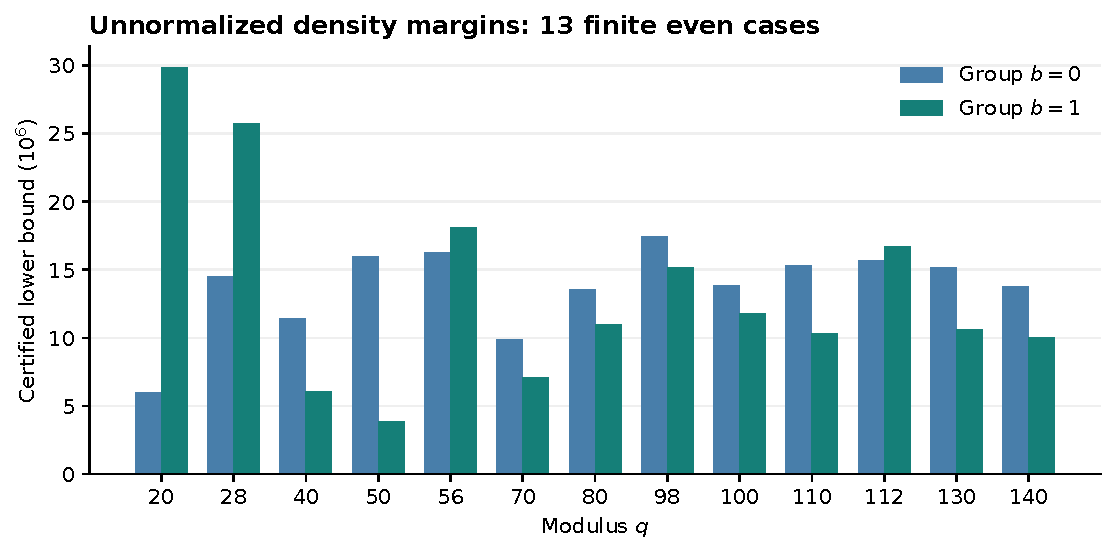
\includegraphics[width=.96\linewidth]{../figures/finite-margins.pdf}\caption{Certified numerator lower bounds for the two positive phase densities at the thirteen finite even moduli. All comparisons use rational arithmetic; plotting uses rounded values.}\label{fig:margins}\end{figure}
\section{Finite grid laws and a uniform margin}
All constructed phase laws have full support (or a positive Haar component). A full-support mean of a continuous vector map on compact $H$ lies in the relative interior of its convex hull: any supporting linear functional saturated at the mean is constant on $H$. For algebraic $\delta>0$, $\delta c\cdot\alpha$ is algebraic and belongs to $2\pi\Z$ only when zero, by transcendence of $\pi$. The character criterion for torus density gives the same closure for $\{t_0+j\delta:j\ge0\}$; positive iterates are dense by recurrence. The convex hull of the grid image is dense in the compact phase convex hull and shares its relative interior \cite[Theorem 6.3]{rockafellar}. Carath\'eodory's theorem then bounds support by the number of real gap characters plus one. The character counts are at most $m^2$ for odd $q$, $m(m+1)$ for even $q$. This completes the proposed proof of Theorem~\ref{thm:main}.
\begin{theorem}[Uniform Haar floor, conditional on the inventories]\label{thm:floor}
Every admitted modulus has a phase law $\nu$ with real target character means and $\nu\ge h/100$.
\end{theorem}
\begin{proof}
In Part I the ratio $(G-E)/(Z+G)>1/100$. In Part II the shifted numerators of $G-E_b-T/100$ (at $b\ge4$) and $G-E_b-E_{\rm extra}-T/100$ (at $b\ge16$) have positive constant and nonnegative coefficients. The exact margins at 33 and 39 exceed $T/100$ and $q=9$ has Haar weight $1/8$. For even groups the same shifted-polynomial check with $\tfrac{99}{100}(-NU)-Z$ in place of $G$, and the exact finite ratios, gives $\nu_b\ge h_b/100$. These rational tests are given in \texttt{verify\_uniform\_floor.py}. To avoid multiplying the two floors, put $c=1/100$, $\rho_b=(\nu_b-ch_b)/(1-c)$ and $\nu=ch+(1-c)\rho_0\times\rho_1$. Nontrivial within-group means are restored by the factor $1-c$; cross means stay zero because the unbiased first moments vanish. For $q=4,5,6,8$ the known phase ramp \cite[Proposition S22]{kang} with $\lambda=1+1/(2N)$ mixed with Haar has weight $1/(2N+1)>c$. The remaining $q=3$ uses Haar. Symmetrizing by inversion preserves the real means and floor.
\end{proof}
Let $\Omega$ be the distinct positive gaps, $y$ the target real means, and $C$ the convex hull of the complex character vector on $H$. For any perturbation $u$ with $\sum_{\omega\in\Omega}|u_\omega|<1/200$, add the signed Haar density $2\Rea\sum_\omega u_\omega\overline{\chi_\omega}$ to $\nu$. This preserves positivity and mass and shifts each complex mean by exactly $u_\omega$. Hence the complex $\ell^1$ ball of radius $1/200$ about $y$ lies in the interior of $C$.
\begin{corollary}[Known timing-noise compensation]\label{cor:noise}
Suppose $X$ is a real, independent timing error of known distribution, finite mean and standard deviation $\sigma\le1/(25\sqrt N)$. Conditional on Theorem~\ref{thm:floor}, a finite planned-time law on any prescribed algebraic-step grid can achieve $\E M(T+X)=J/N$.
\end{corollary}
\begin{proof} Center $X$ by its mean $\mu_X$ and let $k_\omega=\E e^{i\omega(X-\mu_X)}$. Taylor's integral remainder gives $|1-k_\omega|\le \omega^2\sigma^2/2\le8\sigma^2$. There are at most $N^2/4$ nonzero target entries, each of magnitude $1/N$. Thus
\[\sum_\omega|y_\omega/k_\omega-y_\omega|\le\frac{2N\sigma^2}{1-8\sigma^2}\le\frac2{621}<\frac1{200}.\]
Translation by $-\mu_X$ on the phase group preserves the interior. The convex grid argument realizes $e^{-i\omega\mu_X}y_\omega/k_\omega$ exactly, and independence restores $y_\omega$ after noise. For complex moment constraints the support bound is $2|\Omega|+1$.\end{proof}
The noise bound is for dimensionless adjacency time; for $JA$ in units $\hbar=1$, scale physical standard deviation by $|J|$. The protocol depends on the noise law. If actual nonnegative times are required, a lower bound on the error and a sufficiently late starting grid are also required. No experimentally practical maximum waiting time is asserted.
\section{Reproducibility, scope and limitations}
The supplement includes the full relation inventories, exact rational tables, symbolic generating functions, and independent enumeration source. Run \texttt{python verification/run\_checks.py} from the repository root after installing the pinned dependency and a C++17 compiler. The release log records eleven scripts rerun on the package; symbolic inequalities, exhaustive bounded integer searches and rational calculations are separated from mathematical arguments. The C++ enumeration is exact on its bounded integer domain. The previous $P_{19}$ Lean files are included solely as historical finite arithmetic certificates; they do not verify this classification or the real-analytic bridge. AI-assisted drafting and computation were used. There has been no independent mathematical peer review. The highest-risk step remains the completeness of the global short-relation inventory; neither successful tests nor a finite collection of examples certifies an arbitrary-modulus theorem. This is a candidate preprint, not a claim of peer-reviewed proof or guaranteed priority. A literature search on 27 November 2026 located no identical complete positive classification; Kang's v1 and his work on strongly regular graphs \cite{kang2} were checked. No public repository has been changed in preparing this release.
\clearpage
\begin{thebibliography}{9}\small
\bibitem{baptista} P. Baptista, G. Coutinho and V. Marques, Unexpected averages of mixing matrices, \emph{Quantum Information Processing} \textbf{23}, 272 (2024). \href{https://doi.org/10.1007/s11128-024-04480-0}{doi:10.1007/s11128-024-04480-0}.
\bibitem{kang} M. Kang, Arithmetic of Bohr frequencies governs uniform mixing in randomly timed quantum spin chains, \href{https://arxiv.org/abs/2609.14463}{arXiv:2609.14463v1} (13 September 2026), in particular S2--S4.
\bibitem{cj} J. H. Conway and A. J. Jones, Trigonometric diophantine equations (On vanishing sums of roots of unity), \emph{Acta Arithmetica} \textbf{30}, 229--240 (1976). \href{https://doi.org/10.4064/aa-30-3-229-240}{doi:10.4064/aa-30-3-229-240}.
\bibitem{lenstra} H. W. Lenstra Jr., Vanishing sums of roots of unity (1979), pp. 249--267, \href{https://pub.math.leidenuniv.nl/~lenstrahw/PUBLICATIONS/1979d/art.pdf}{author-hosted scan}, especially Theorems 2.2, 2.3 and 2.6.
\bibitem{rockafellar} R. T. Rockafellar, \emph{Convex Analysis}, Princeton University Press (1970), Theorems 6.3 and 17.1.
\bibitem{godsil} C. Godsil, Average mixing of continuous quantum walks, \emph{J. Combin. Theory Ser. A} \textbf{120}, 1649--1662 (2013). \href{https://doi.org/10.1016/j.jcta.2013.05.006}{doi:10.1016/j.jcta.2013.05.006}.
\bibitem{kang2} M. Kang, Moment methods for uniform average mixing on strongly regular graphs, \href{https://arxiv.org/abs/2610.10017}{arXiv:2610.10017} (2026).
\end{thebibliography}
\end{document}
